\chapter{Motivation}
%\setcounter{equation}{0}
%\setcounter{figure}{0}
%\renewcommand{\theequation}{\thechapter.\arabic{equation}}
%\renewcommand{\thefigure}{\thechapter.\arabic{figure}}
	A~\acf{TPC}~\cite{nygren} is a~gaseous detector that reconstructs charged particle trajectories by measuring the positions and drift times of ionization electrons (and sometimes also ions) created in the gas. The energies of these particles can be inferred from the curvatures of their trajectories in a~magnetic field.
	
	The goal of this thesis is to develop an algorithm for the reconstruction of charged particle trajectories and energy in an \emph{atypic} \ac{TPC} with orthogonal electric and magnetic fields, hereafter referred to as the \ac{OFTPC}, used in the X17 project at the \ac{IEAPCTU}. Furthermore, we present the results of testing several (gradually improving) developed algorithms with different samples of simulated data.
	
	The X17 project in \ac{IEAPCTU}~\cite{x17_utef} aims to reproduce measurements of anomalous behavior in the angular correlation distribution of pairs produced by the \ac{IPC} mechanism~\cite{IPC} during the decay of certain excited nuclei (\iso{Be}{8}~\cite{atomki_be,atomki_be2}, \iso{C}{12}~\cite{atomki_c}, and~\iso{He}{4}~\cite{atomki_he,atomki_he2}) observed by a~team at ATOMKI in Hungary.
	
	\section{ATOMKI Anomaly}
	\label{sec:ATOMKI}
		Many different theories propose the existence of \emph{new light boson(s)} that are weakly coupled to ordinary matter~\cite{dark}. These particles are potential dark matter candidates and could contribute to a~solution of other issues with the Standard Model, such as the strong CP~problem\footnote{The CP symmetry could be violated in strong interactions according to the current formulation of quantum chromodynamics, but no such violation is observed.} and the anomalous muon magnetic moment.
		
		A~possible way of detecting such bosons with a~short lifetime is to observe nuclear transitions of excited nuclei. If a~boson was emitted during the transition and subsequently decayed into an electron\nobreakdash-positron pair, we could observe this as a~peak on top of the standard $e^+e^-$ angular correlation from the \acf{IPC} and the \acf{EPC}.
	
		\subsection{ATOMKI Measurements}
			Historically, there were several measurements of the \ac{IPC} in nuclear transitions in~\iso{Be}{8} at Institute für Kernphysik (Frankfurt)~\cite{ikf1996,ikf1997,ikf2001} and at ATOMKI (Debrecen, Hungary)~\cite{atomki2008,atomki2012} resulting in different anomalies with invariant mass in the range \qtyrange{5}{15}{\MeV}. This motivated the development of a~better spectrometer at ATOMKI.
		
			In 2015, a~group at ATOMKI observed an anomalous~\ac{IPC} in~\iso{Be}{8}~\cite{atomki_be}. They used the \iso{Li}{7}$(p,\gamma)$\iso{Be}{8} reaction at the $E_p = \qty{1030}{\keV}$ proton capture resonance to prepare the \qty{18.15}{\MeV} excited state ($J^\pi = 1^{+}$, $T=0$). This state decays predominantly through M1~transitions to the ground state ($J^\pi = 0^{+}$, $T=0$) and to the \qty{3.03}{\MeV} state ($J^\pi = 2^{+}$, $T=0$)~\cite{resonances}.
			
			The angular correlation of the $e^+ e^-$ pairs created internally in these transitions were measured and compared to the simulation; results from a~narrow $E_\text{sum}=18$~MeV region are shown in \cref{fig:atomki_be}. The simulation includes boson decay pairs for different boson masses. The disparity parameter~$y$ is used to describe the asymmetry of energy between the two particles. It is defined as
				\begin{equation}
					\label{eq:dispar}
					y = \frac{E_{e^-}-E_{e^+}}{E_{e^-}+E_{e^+}},
				\end{equation}
			where $E_{e^-}$ and $E_{e^+}$ are the kinetic energies of the electron and positron.
			
			Their experimental setup was later upgraded and used for new measurements. In 2022 the \iso{Be}{8} anomaly was also measured using the $E_p = \qty{441}{\keV}$ resonance to produce the \qty{17.64}{\MeV} excited state ($J^\pi = 1^{+}$, $T=1$) which again decays primarily to the ground state and the \qty{3.03}{\MeV} state~\cite{resonances}. The anomaly was also verified for $E_p = \qtylist{650;800}{\keV}$ where E1~transitions from the direct proton capture dominate~\cite{atomki_be2}. The results for $e^+e^-$ with ${E_\text{sum}\in[13.5,20]}$~MeV are shown in \cref{fig:atomki_be2}.
			
			The newer setup was also used in 2021 to study the \iso{H}{3}$(p,e^+ e^-)$\iso{He}{4} reaction at $E_p = 510$, 610 and 900~keV~\cite{atomki_he2}, inducing direct and resonant capture populating the overlapping first 20.21~MeV ($J^\pi = 0^+$) and second 21.01~MeV ($J^\pi = 0^-$) excited states~\cite{resonances2}. The comparison of simulated and measured $e^+e^-$ pair angular correlations in the ${E_\text{sum}\in[18,22]\,\unit{\MeV}}$ region is shown in \cref{fig:atomki_he}.
			
			In 2022, another anomaly was measured in the \iso{B}{11}($p,e^+e^-$)\iso{C}{12} process~\cite{atomki_c}. The $E_p = \qty{1388}{\keV}$ resonance was used to populate the \qty{17.23}{\MeV} excited state ($J^\pi = 1^-$, $T = 1$) with a~large width $\Gamma = \qty{1.15}{\MeV}$~\cite{resonances3}. This state decays mainly through E1~transitions to the ground state $J^\pi = 0^+$ and to the \qty{4.44}{\MeV} state $J^\pi = 2^+$. To compensate for energy losses in the target, five energies in the range $E_p = \qtyrange{1.5}{2.5}{\MeV}$ were used. The experimental angular correlation for the \qty{17.23}{\MeV} transition to the ground state is shown in \cref{fig:atomki_c}.
			
				\begin{figure}
					\centering
					\begin{subfigure}[t]{0.48\textwidth}
						\centering
						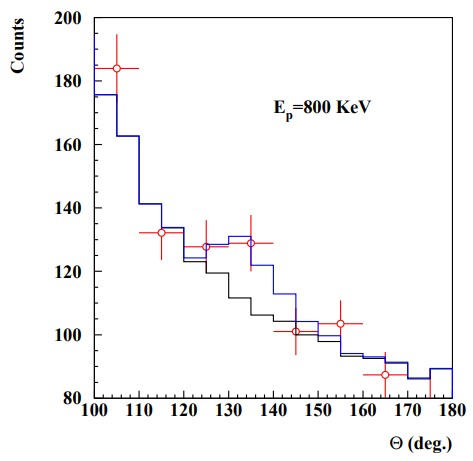
\includegraphics[width=\textwidth]{atomki_be.png}
						\caption{Experimental $e^+e^-$ pair correlations measured in the \iso{Li}{7}$(p,e^+e^-)$\iso{Be}{8} reaction with $|y| \leq 0.5$ (closed circles) and $|y| \geq 0.5$ (open circles)~\cite{atomki_be}.}
						\label{fig:atomki_be}
					\end{subfigure}
					\hfill
					\begin{subfigure}[t]{0.42\textwidth}
						\centering
						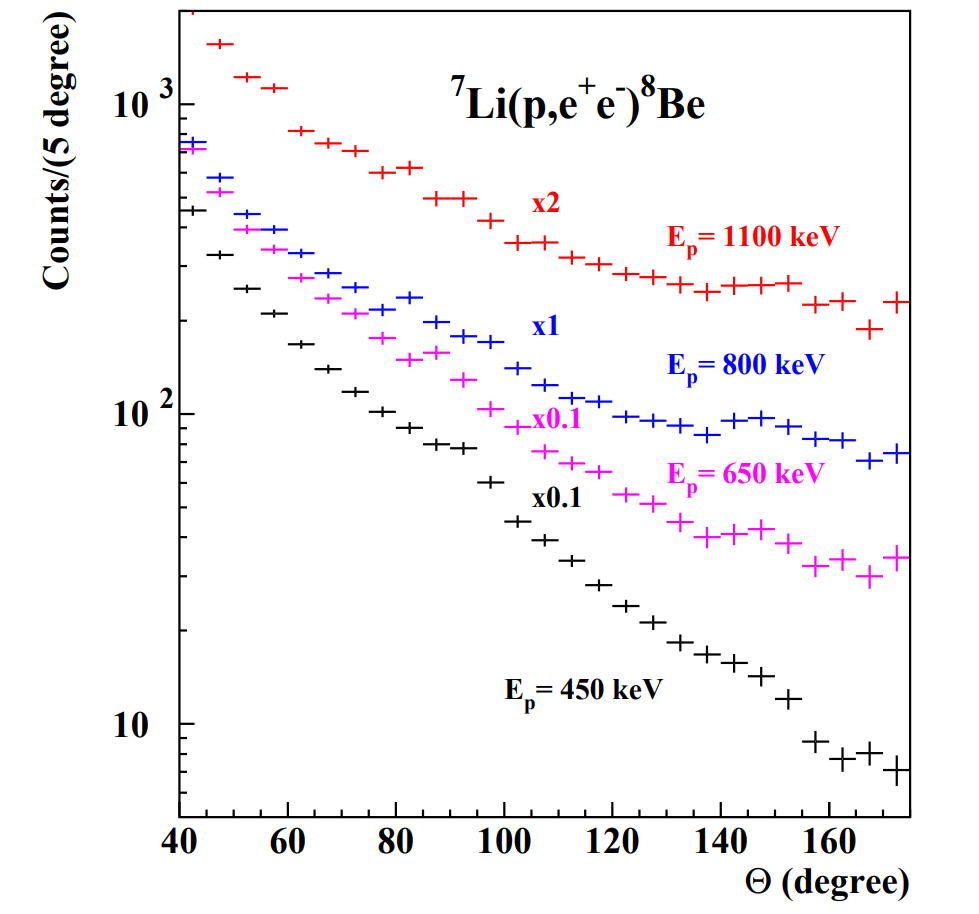
\includegraphics[width=\textwidth]{atomki_be2.png}
						\caption{Experimental $e^+e^-$ pair correlations measured in the \iso{Li}{7}$(p,e^+e^-)$\iso{Be}{8} reaction with the improved setup for different proton beam energies~\cite{atomki_be2}.}
						\label{fig:atomki_be2}
					\end{subfigure}
					\begin{subfigure}[t]{0.45\textwidth}
						\centering
						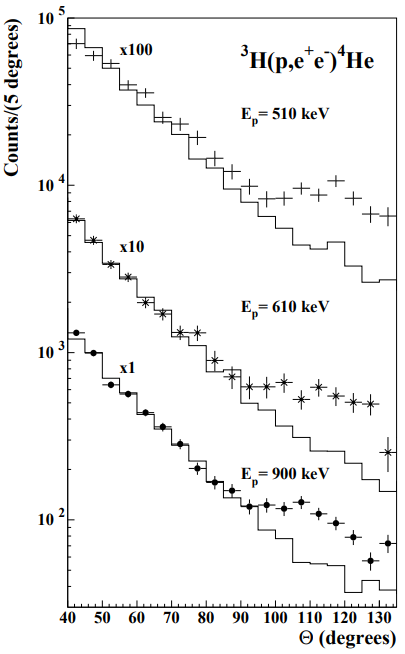
\includegraphics[width=\textwidth]{atomki_he.png}
						\caption{Experimental $e^+e^-$ pair correlations measured in the \iso{H}{3}$(p,e^+e^-)$\iso{He}{4} reaction with $|y| \leq 0.3$ for different proton beam energies~\cite{atomki_he2}.}
						\label{fig:atomki_he}
					\end{subfigure}
					\hfill
					\begin{subfigure}[t]{0.45\textwidth}
						\centering
						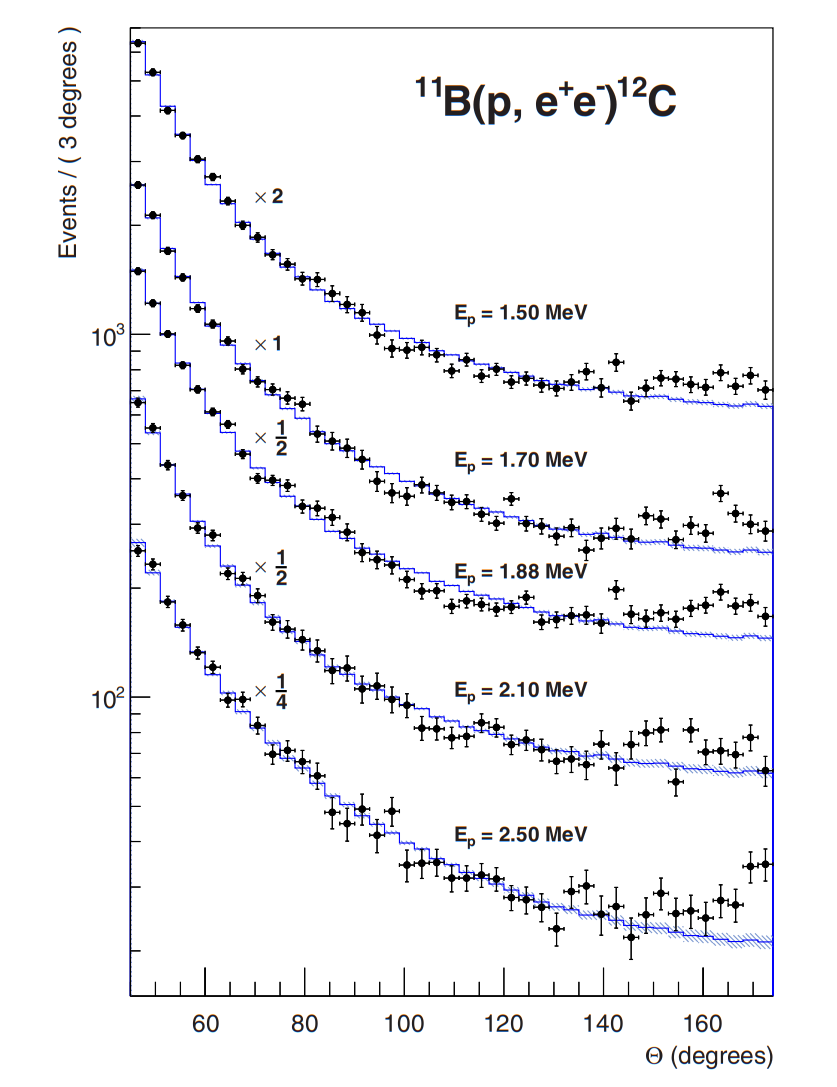
\includegraphics[width=\textwidth]{atomki_c.png}
						\caption{Experimental $e^+e^-$ pair correlations measured in the \iso{B}{11}$(p,e^+e^-)$\iso{C}{12} reaction for different proton beam energies~\cite{atomki_c}.}
						\label{fig:atomki_c}
					\end{subfigure}
					\caption{The ATOMKI anomalous \ac{IPC} measured for different nuclei.}
					\label{fig:atomki}
				\end{figure}
			
				Possible explanations of the anomaly include experimental effects, higher order processes in the Standard Model~\cite{kalman,aleksejevs} or even a~protophobic fifth force mediated by a~new \qty{17}{\MeV} boson X17~\cite{feng}.
		\subsection{Other Experiments}
			Since the ATOMKI measurements, several experiments have been initiated to attempt to replicate the results and search for the hypothetical X17 particle. The following experiments have already produced results~\cite{atomki_review}.
			
			\subsubsection{Two-arm $e^+e^-$ spectrometer in Hanoi}
				The anomaly in \iso{Be}{8} has been observed with a~high ($>4\sigma$) confidence by a~team at the Hanoi University of Sciences for $E_p = \qty{1225}{\keV}$~\cite{hanoi}. They built a~two\nobreakdash-arm spectrometer in collaboration with ATOMKI and calibrated it using the \qty{17.6}{\MeV} M1 transition. The results are shown in \cref{fig:hanoi}.
				
				\begin{figure}
					\centering
					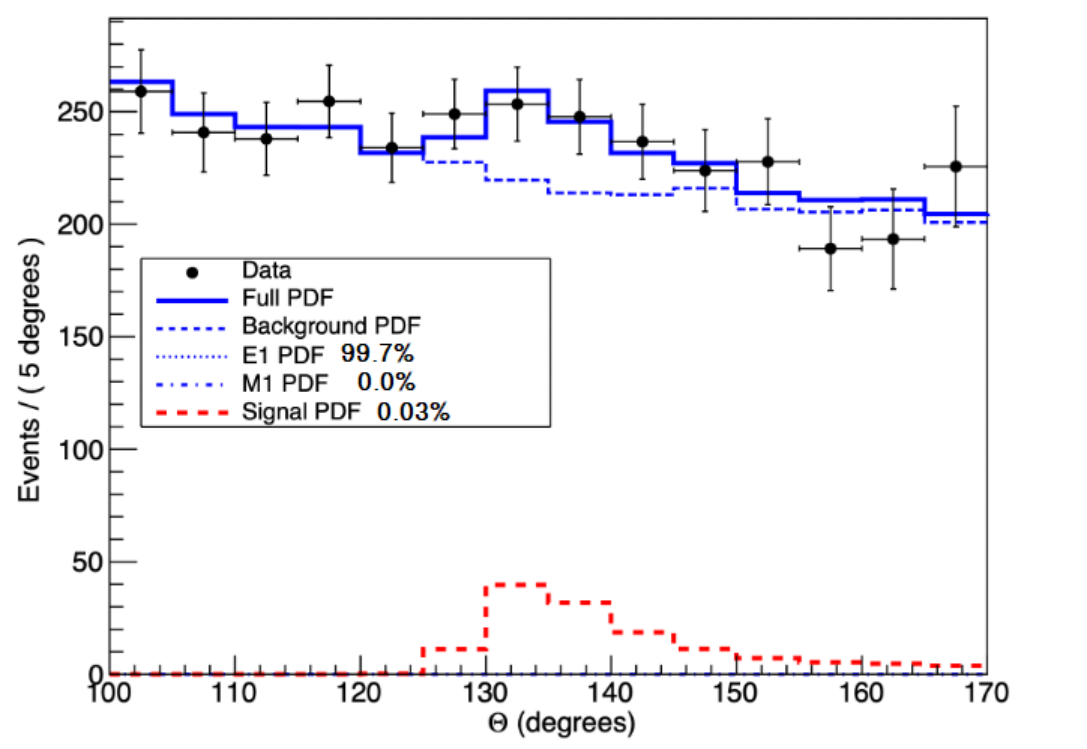
\includegraphics[width=0.75\textwidth]{hanoi.png}
					\caption{Results from the Hanoi spectrometer - angular $e^+e^-$ pair correlations measured in the \iso{Li}{7}$(p,e^+e^-)$\iso{Be}{8} reaction at $E_p = \qty{1225}{\keV}$~\cite{hanoi}.}
					\label{fig:hanoi}
				\end{figure}
			
			\subsubsection{Collisions at Nuclotron in Dubna}
				At the Joint Institute for Nuclear Research in Dubna, signal in the form of enhanced structures in the $\gamma\gamma$ spectra at \textapprox17 and \textapprox38~MeV invariant masses for $p+\mathrm{C}$, $d+\mathrm{C}$ and $d+\mathrm{Cu}$ reactions at momenta 5.5, 2.75, and 3.83~GeV per nucleon~\cite{dubna}. Monte Carlo simulations support the conclusion that the signals are a~consequence of a~decay of unknown particles X17 and E38.
				
			\subsubsection{The MEG II (Muon Electron Gamma) experiment}
				Experiments using the \iso{Li}{7}$(p,e^+e^-)$\iso{Be}{8} reaction were carried out at the Paul Scherrer Institute with the MEG II superconducting solenoid spectrometer~\cite{megii}. Analysis of the data with $E_p = 1080$~keV exciting both of the resonances (beam fully stopping in the target) found no significant evidence supporting the X17 hypothesis, results are shown in \cref{fig:megii}. An upper bound (at 90\% confidence) on the X17\nobreakdash-to\nobreakdash-$\gamma$ branching ratio was set at $1.2\cdot10^{-5}$ for the 18.15~MeV state (larger than the ratio $5.8\cdot10^{-6}$ obtained by ATOMKI in 2016).
				
				\begin{figure}
					\centering
					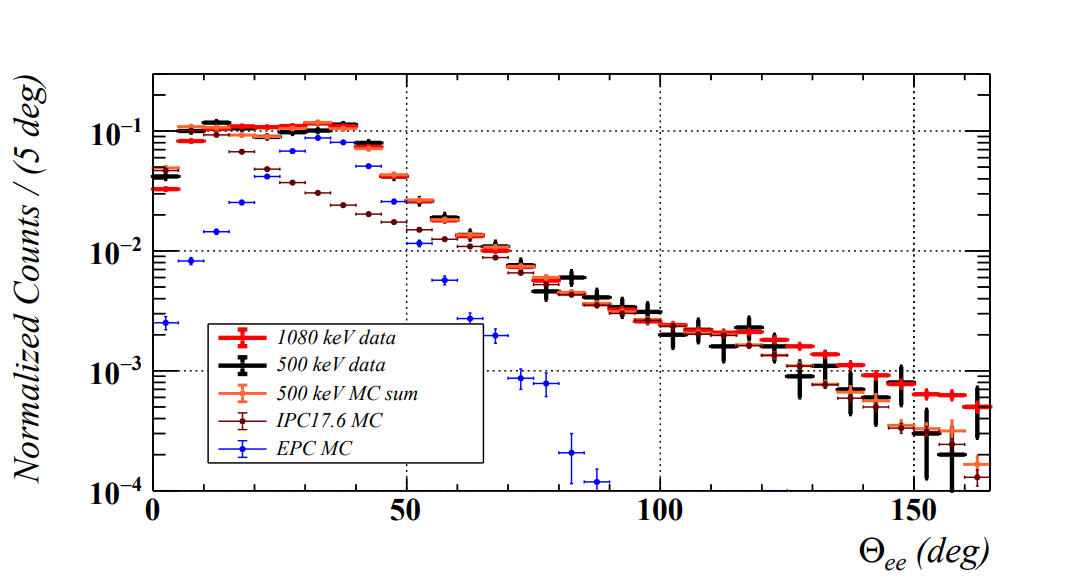
\includegraphics[width=0.9\textwidth]{megii.png}
					\caption{Results from the MEG II experiments -- angular correlation of $e^+e^-$ pairs with $E_\text{sum} \in [16,20]$~MeV measured in the \iso{Li}{7}$(p,e^+e^-)$\iso{Be}{8} reaction with proton beam energies 500 and 1080~keV. The 500~keV dataset is fitted with Monte Carlo of both the \ac{IPC} deexcitation and the \ac{EPC} produced by gammas~\cite{megii}.}
					\label{fig:megii}
				\end{figure}
			
	
	\section{X17 Project at IEAP CTU}
	\label{sec:IEAP}
		The aim of the X17 project at the Van der Graaff facility of the \acl{IEAPCTU} is to reproduce the results of the original ATOMKI experiments with \iso{Li}{7} and \iso{H}{3} targets using an independent $e^+e^-$ spectrometer. In order to effectively measure the anomaly, we need to reconstruct both the energy and the angular correlation of the $e^+e^-$ pairs. The spectrometer will use three layers of detectors to achieve this -- \acf{TPX3} silicon pixel detector and \acf{MWPC} layers for the angle reconstruction and a~\acf{TPC} layer for the energy reconstruction. The schematics of the prepared detector is in \cref{fig:ieap}.
			
			\begin{figure}
				\centering
				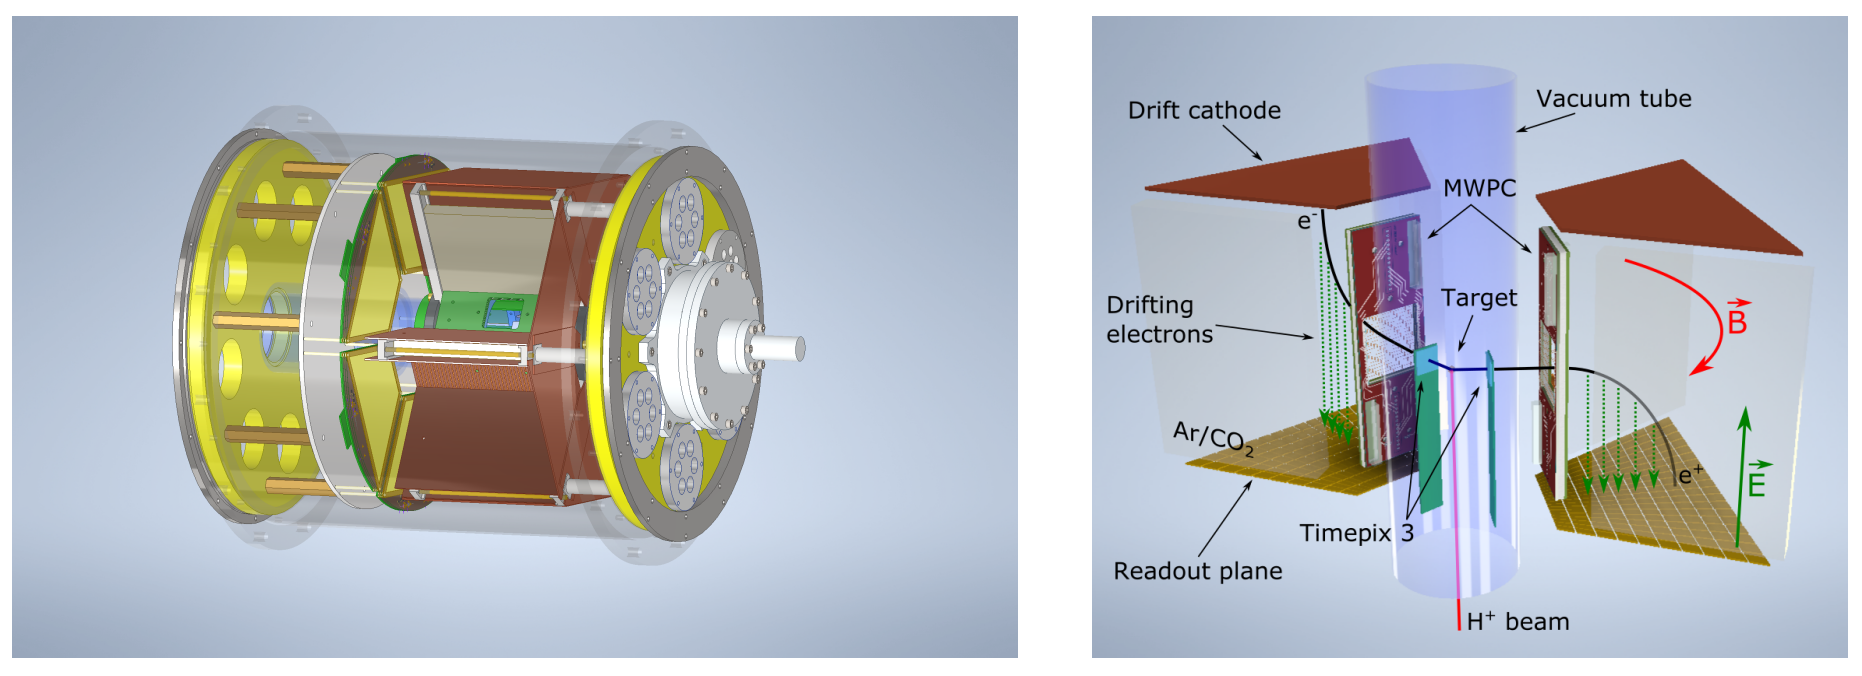
\includegraphics[width=\textwidth]{ieap_x17.png}
				\caption{Schematics of the detector at the Van der Graaff facility at~\ac{IEAPCTU}~\cite{x17_utef}.}
				\label{fig:ieap}
			\end{figure}
		
		The energy of $e^+e^-$ pair produced in the reaction is given by the energy available $E_\text{r}$ in the reaction and can be distributed between them arbitrarily. Nonetheless in the decay of the hypothetical X17 particle, electron and positron should have similar energy and we can therefore use a~cut $|y| \leq 0.5$ in the disparity parameter (defined in \cref{eq:dispar}). Interesting events should rarely have a~particle with an energy below $E_\text{r}/4$ (roughly \qty{4}{\MeV}). Electrons with such low energies are scattered significantly by even a~thin layer of relatively light material, for this reason the \ac{TPX3} layer will be inside of the vacuum tube and the tube will have a~thinned aluminum segment or Kapton\texttrademark\ windows.
		
		\ac{TPX3} can measure (in each \qtyproduct{55x55}{\um} pixel of its \numproduct{256x256} grid) \ac{ToA} with \qty{1.6}{\ns} precision and \ac{ToT} which reflects the deposited energy. This potentially allows 3D~tracking if we increase the chip thickness at the cost of increased scattering. The layer can reconstruct the reaction vertex and the angular correlation with high precision. Preparatory studies of the angular correlation reconstruction~\cite{triangle}, and energy deposition in the sensor~\cite{tpx3_tracks} have been made.
		
		The layer of \acp{MWPC} with sensitive area \qtyproduct{40x38}{\mm} will be outside of the beam pipe. It will provide an extra point on the particle trajectory which can help with the estimation of the reaction vertex and improve the \ac{TPC} performance by providing its entry point.
		
		The \acp{TPC} that are the subject of this thesis, are in a~magnetic field generated by permanent magnets positioned between them and provide 3D track reconstruction and subsequent momentum and particle identification (its charge, or even type based on its stopping power). They avoid radiative losses thanks to the low density and atomic number of the gas mixture. For the readout, triple \ac{GEM} will be used. The magnetic field layout in our \acp{TPC} is atypical -- orthogonal to the electric field inside the chamber, this is why we call them \acf{OFTPC}. Further details about our \acp{OFTPC} are provided in \cref{sec:oftpc}.